\documentclass{article}
\usepackage{graphicx}
\usepackage{amsmath}

\usepackage{subcaption}
\begin{document}
	
	\title{Introduction to Circuitry}
	\author{}
	
	\maketitle
	
	\begin{abstract}
	In this article we will have an in-depth look at some of the math  necessary for circuit analysis, namely exponential function and natural logarithm. We also see their uses in a simple circuit as well.
	\end{abstract}
	
	\section{Natural Logarithm}
	Let's find a function that would satisfy the following equation:
	
	\begin{equation}
	\label{simple_equation}
	f(ax) = f(a) + f(x)
	\end{equation}
	
	($f$ as function of $x$ and $a$ as an arbitrary constant.)
	
	
	Why do we want such a function? Because it has numerous important properties that we will discuss later in this document.
	For now let's continue finding such a function. A function $f$ that would satisfy an equation such as above, could have many different forms and finding them all would be a difficult or even an impossible task. What we want to do instead, is to add more properties to the equation that would narrow down the function we are looking for. The first property is that we don't want $f$ to be a function that maps all of its inputs to $0$; Because such a function \textit{would} satisfy the equation (1), but it wouldn't be useful at all. The next important property that we want to add which makes a lot sense too, is to find an $f$ that would be continuous and differentiable. In other words, Finding an $f$ that would make the derivative (in respect to $x$) of the right-hand side and left-hand side of equation (1), equal. If we find such a function $f$ such that $\frac{d}{dx}f(ax)$ gives \textbf{equal} values as $\frac{d}{dx}(f(a) + f(x))$ for a range of inputs, we can use the fundamental theorem of Calculus to find the $f$ itself. The function $f$ found in this procedure not only could be an answer for equation (1), moreover it would be differentiable for that range of the values of $x$.	
	Now to find such a function let's differentiate both sides of equation (1). We get:
	
	$$ \frac{d}{dx} f(ax) = \frac{d}{dx} f(a) + \frac{d}{dx} f(x) $$
	
	Now $\frac{d}{dx} f(a)$ is just $0$ (because it's not a function of $x$), therefore we get:
	
	$$ \frac{d}{dx} f(ax) = \frac{d}{dx} f(x) $$
	
	What function $f$ would make the above equation valid? Let's differentiate left side and see what we get. By implicit differentiation:
	
	$$ \frac{d}{dx} f(ax) = \frac{d}{dx} ax \frac{d}{dx} f(ax) = a \frac{d}{dx} f(ax) $$
	
	Now if $$\frac{d}{dx} f(ax) $$ yields the reciprocal of it's argument $ax$, namely $\frac{1}{ax}$ then:
	
	$$ \frac{d}{dx} f(ax) =  a . \frac{1}{ax} = \frac{1}{x} = \frac{d}{dx} f(x) $$
	
	We now know the \textit{derivative} of $f$ should give the reciprocal of it's argument, then $f$ itself is the \textit{integration} of the reciprocal of it's argument:
	
	$$f(x) = \int_{c}^{x} (1/t) dt$$
	
	We are almost there. To recap, the function $f$ that we got so far has the following property:
	
	$$ \frac{d}{dx} f(ax) = \frac{d}{dx} f(x) $$
	
	However, we initially differentiated the equation (1) and we got to this function so far. If the equation had \textbf{any other} constant beside $ln(a)$, it would still cancel out in the differentiation process. So by the (second) fundamental theorem of Calculus, integrating both sides, give the functions \textit{plus} some constant that it could have any value. Therefore for the function we got so far:
	
	$$ f(ax) = f(x) + C $$
	
	For some constant $C$. However if we define $f$ as the integral of $1/t$ from \textbf{"\boldmath{$1$} to \boldmath{$x$}}"  instead of an \textbf{"arbitrary \boldmath{$c$} to \boldmath{$x$}"}, namely:
	
	$$f(x) = \int_{1}^{x} (1/t) dt$$
	
	Not only the derivative of $f(ax)$ would equal to derivative of $f(x)$, moreover:

	$$ f(ax) = f(x) + f(a)$$
	
	Because by letting $x = 1$ we get:
	
	$$ f(a) = f(1) + C$$
	$$ f(a) = 0 + C$$
	$$ f(a) = C $$
	
	And $f(ax)$ for other $x$s besides $x = 1$ would still give this constant - which is equal to $f(a)$ - plus $f(x)$. We are now done.
	
	Such a function has a special name in math and its called \textbf{natural logarithm} and it's denoted by $ln$:
	
	\begin{equation}
	ln(x) = \int_{1}^{x} (1/t) dt
	\end{equation}

	\subsection{Logarithm in "other bases"}
	
	If $b > 0$, $b \neq 1$ and if $x > 0$, the logarithm of $x$ to the "base" $b$ is defined as:
	
	$$ \log_b x = \frac{ln x}{ln b} $$
	
	A common base $b$ is 10. Example:
	
	$$ \log_{10} 1000 = \frac{ln 1000}{ln 10} = \frac{\ln (10 * 10 * 10)}{ \ln 10} = \frac{3 \ln 10}{\ln 10} = 3 $$
	
	or for example another widely used base, logarithm in base 2:
	
	$$ \log_{2} 8 = \frac{ln 8}{ln 2} = \frac{\ln (2 * 2 * 2)}{ \ln 2} = \frac{3 \ln 2}{\ln 2} = 3 $$
	
	\section{The constant $e$}
	The constant $e$ is a number that we define as the value in which $\ln(e) = 1$. Plugging it in the definition of the natural logarithm, it means it's a number which the area under the curve of $\frac{1}{x}$ \textit{from $1$ to that number $e$} is 1.
	

	Now a property of natural logarithm that we left out is the following property, for a \textit{rational} $n$:
	
	$$ \ln(x^n) = n\ln(x) $$ 
	
	Proof (by power rule):
	
	$$ \frac{d}{dx} \ln(x^n) = \frac{1}{x^n} . \frac{d}{dx} x^n = \frac{n}{x^n} . x^{n-1} = \frac{n}{x} = n \ln x$$
	
	Even though the following property is true only for the rational powers of $x^n$, we can "fill in" for the irrational numbers as well. By defining the output for the irrational powers as the limit approaching to the closest neighboring rational power. Graphically we fill in the wholes in the graph for irrational numbers.
	
	To recap, we have found a function and we called it $\ln(x)$ which has the following properties:
	\begin{flalign*}
	& 1) \; \ln(ax) = \ln(a) + \ln(x) &\\
	& 2) \;\; (\ln x)' = \frac{1}{x} &\\
	& 3) \; \ln(x^n) = n \ln x &
	\end{flalign*}
	
	Now we want to find the \textit{inverse} of the natural logarithm. To do so, what expression should we give to the natural logarithm that it would give us the term $x$ itself? Such an expressions would be the inverse of the natural logarithm. This expression is $e^x$; Because:
	
	$$ \ln e^x = x \ln e = x $$
	
	Therefore, $e^x$ is defined as the inverse of the natural logarithm:
	
	$$ e^x = \ln ^{-1} x $$
	
	Now we will discover one of the most significant mathematical properties of this function, which appears frequently in the universe.
	
	\section{The Function $\mathbf{e^x}$}
	The function $e^x$ has numerous important properties. One of the most important ones, which we use over and over in circuitry and other fields as well is \textit{the derivative of the function $e^x$ which is $e^x$ itself}.
	
	
	Proof:
	$$ y = e^x $$
	
	Therefore (by the 3nd property of $\ln$):
	
	$$ \ln e^x = x $$

	Taking implicit differentiation of both-sides (by the 2nd property of $\ln$):
	
	$$ \frac{d}{dx} \ln y = \frac{d}{dx}x $$
	$$ \frac{1}{y} \frac{d}{dx} y = 1$$
	
	Finally:
	$$\frac{d}{dx} y = y$$
	
	Which means:
	
	\vspace{5mm}
	
	\begin{equation}
	\frac{d}{dx} e^x = e^x
	\end{equation}
	
	\vspace{5mm}
	
	This function is called the exponential function and is also denoted by \boldmath$\exp(x)$. This function is the solution to \textit{$y' = y$}. In other words, what function gives the same values as it's instantaneous rate of change? $e^x$.
	
	Concept of logarithms and exponential function could be approached in many different ways. One can differentiate the function $a^x$ via plugging it into the definition of the derivative. Using this method we get a function times a weird-looking limit. Thus continuing to prove that this limit is the inverse of the famous constant $e$ to the power of $a$; Then we shall call this inverse function as the logarithm in base $e$. Another way which we used in this article is by defining the logarithm \textit{first} then defining the constant $e$ as a number that if we give to the natural logarithm, it yields $1$. Anyhow all the different ways lead to the same concepts but we used the latter one which we think is the right way to explain these topics.
	
	\subsection{Applications of the Function $e^x$}
	We now examine a case which the exponential function appear in circuit analysis. Assume a simple circuit consisting of a battery, a resistor and an inductor. And they are all connected in series and has the value as shown in the following schematic:
	\begin{figure}[h!]
 	\centering
	\begin{subfigure}[b]{0.6\linewidth}
		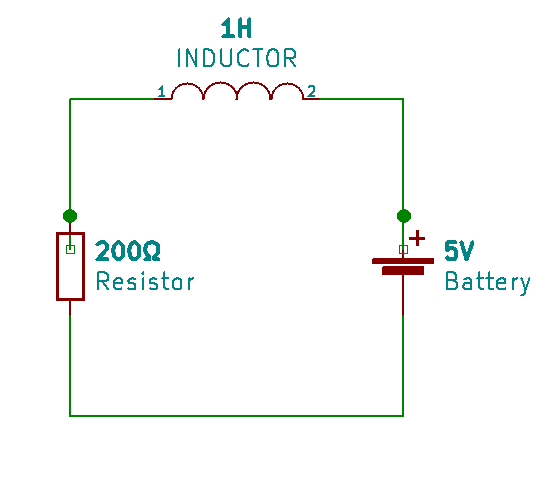
\includegraphics[width=\linewidth]{circuit1.png}
	\end{subfigure}
	\end{figure}
	
	We now want to analyze this circuit; This means that our goal is to find the voltage drops (of each element) and the currents flowing through each loop. For analyzing this circuit we use the laws that come from the nature. Namely, conservative of energy (which is called KVL in circuit analysis), Ohm's law and the formula for induced voltage of an inductor. Let's start analyzing this circuit step-by-step.
	
	By the law of conservation of energy, adding up the voltage drops of each element should sum up to zero. This means:
	
	$$V_{battery} + V_{resistor} + V_{inductor} = 0$$
	
	Now this let's substitute corresponding values of each term. Voltage drop across a battery is constant over time and in this example is 5; Let's denote this constant $\varepsilon$ for a general battery. Therefore $V_{battery} = \varepsilon$. For the resistor by Ohm's law, voltage drop across the resistor should be proportional to a constant, times the current flowing through it: $V_{resistor} = Ri$. As for the inductor, voltage drop across it is proportional to a constant times the \textit{instantaneous rate of change} of it's current over time\footnote[1]{The exact reason why the induced voltage of an inductor (or more generally Faraday's law of induction) is proportional to rate of change of it's current over time comes from a more general theory which is the "theory of relativity". We shall discuss these topics in the later articles in-details. But in basic terms when electrons gain speed they (and space between them) gets contracted; Thus producing "magnetic effect". Changing of this magnetic effect causes instant accumulation of electrons which EMF gets produced.}. Hence: $V_{inductor} = L\frac{di}{dt}$. Now let's plug all of these into the equation. 
	
	$$\varepsilon - Ri(t) - L\frac{di}{dt} = 0 $$
	
	Bringing $-L\frac{di}{dt}$ to the other side we get:
	
	$$\varepsilon - Ri(t) = L\frac{di}{dt} $$
	
	Now here comes the interesting part. Let's take the whole expression on the left-hand side as a single term and call it $U$. Therefore:
	
	$$ U = \varepsilon - Ri(t) $$
	
	Taking a look at this expression, we see $\varepsilon$ term is just a constant, therefore the $U$ is merely a function of $i$ over time. On the right-hand side we have the derivative of $i$ over time! (times a constant $L$ too). Essentially what we have here is a function on one side and it's derivative on the other side. To find this $U$ we simply have to look at a function \textit{whose value at different inputs, are same as it's derivative at those points}. This is were exponents come to play.
	Solving this equation, we get:
	
	\begin{equation}
	 	i(t) = \frac{\varepsilon}{R}(1 - e^{-(R/L)t})
	\end{equation}
	
	By the way, the exact steps of how we got to this expression is omitted; They are merely algebraic manipulations for solving these differential equations. The important part is that this function is in form of exponential function $e^x$.
	
	To recap what really happened, we know by the physical property of an inductor that the voltage drop across it, is proportional to the rate of change of it's current over time. And this value, because of the conservation of energy, should be equal to the voltage gain/drop of the battery plus the resistor. The voltage gain of battery is just a fixed number over time; But for the resistor we know from Ohm's law that the voltage drop across it is linearly proportional (approx. for a real resistor) to it's current. So from putting these facts together, we are looking for a set of values over time in which their instantaneous rate of change is the same as their own values at those points.
	
	Finally substituting values of $\varepsilon$, $R$ and $L$ for this into this equation we get:
	
	$$ i(t) = 0.05(1 - e^{-(100)t})  $$
	
	Plotting this function we get:
	\begin{figure}[h!]
		\centering
		\begin{subfigure}[b]{0.9\linewidth}
			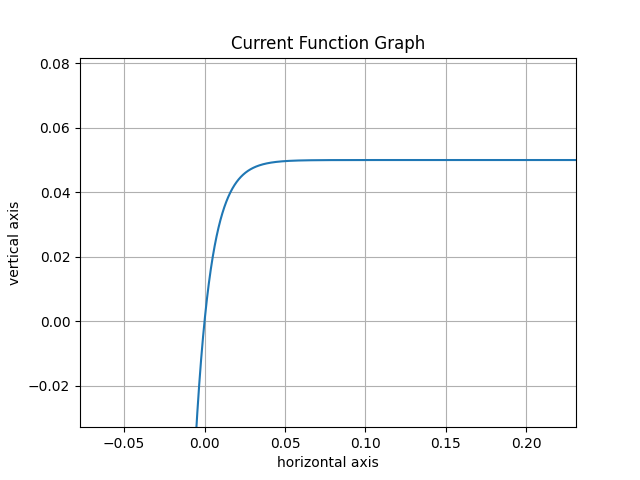
\includegraphics[width=\linewidth]{Figure_1.png}
		\end{subfigure}
	\end{figure}

	Similar situation would happen if we had a capacitor instead of an inductor. With the difference that the part in which the derivative appears (in this case derivative of charge $Q$ over time instead of current $i$ over time), would be for the resistor. Namely, if we had a capacitor instead of an inductor in this circuit, we should have gotten:
	
	$$\varepsilon - Ri(t) - \frac{Q}{C} = 0 $$
	
	Because the voltage drop across a capacitor is proportional to the accumulated charges $Q$ in one plate over a constant $C$ (capacitance). And that number, should be equal to the resistivity  $R$, times the current for the resistor part (Ohm's law). Current by definition is just the change of $Q$ overtime ($i(t) = \frac{dq}{dt}$). Consequently, solving that differential equation should give us the change of $Q$ over time (instead of $i$) as an exponential.
	
	In future tutorials we shall discuss and analyze the circuits consisting of both capacitor and inductor beside resistors and power supplies. For now, our goal was to get the big picture of the math behind this circuits and solve a basic one.
	
	\section{What's Next?}
	In the follow up article, we will discuss some math behind the circuitry consisting of sinusoidal signals; Namely Phasor Digarams and also the definition Root Mean Square (RMS) and to see why is's convenient to define such an expression in AC circuits.
	
	These documents are published under open license and were intended to be part of an open and a collaborative project. Feel free to fork this document, send pull request and also give your feedback. Thanks for reading!
	
\end{document}
